
\section{Experiments}
\label{sec:experiments}




\subsection{Experimental Setup}
We evaluate our proposed method on the \textbf{Wan2.2}~\cite{wan2025wan} T2V and I2V models at 480P resolution with 81 frames (40 sampling steps), and the \textbf{HunyuanVideo}~\cite{kong2024hunyuanvideo} T2V model at 480P resolution with 129 frames (50 sampling steps). Our evaluation dataset comprises diverse prompts curated from the official Wan2.2, Wan-Lightning~\cite{fan2025wanlighting}, and Open-Sora~\cite{zheng2024opensora} example sets, following the evaluation protocol of SageAttention~\cite{zhang2025sageattention1}. For the attention mechanism, we employ \textbf{per-token quantization} for the query ($\mathbf{Q}$) and key ($\mathbf{K}$) matrices, and \textbf{per-group quantization} for the value ($\mathbf{V}$) matrix.

For \textbf{Wan2.2-I2V}, we preserve FP16 precision for the first 6 and last 4 sampling steps, as well as the first and last 2 DiT blocks; all remaining FlashAttention operations are executed with our INT4 attention kernel, resulting in 68\% of FlashAttention operations running in INT4. For \textbf{Wan2.2-T2V}, FP16 is maintained for the first and last 2 sampling steps and DiT blocks, enabling 81\% INT4 attention execution. Similarly, for \textbf{HunyuanVideo-T2V}, we keep FP16 for the first 4 and last 2 sampling steps and the first and last 2 DiT blocks, with 76\% of attention operations running in INT4.

\paragraph{\textbf{Hardware Configuration.}} We benchmark INT4 attention kernel speed on \textbf{NVIDIA A10} GPUs using custom CUDA kernels, reflecting practical deployment hardware. For accuracy evaluation of the full video generation pipeline, we use \textbf{NVIDIA H20} GPUs with \textbf{TileLang}~\cite{wang2025tilelang} operators, which provide precise numerical validation. 


\paragraph{\textbf{Model Scope.}} We evaluate on Wan2.2 and HunyuanVideo, two leading open-source video generation models, both employing DiT-based architectures with 3D RoPE. This choice is deliberate: DiT with 3D RoPE has become the \emph{de facto} standard for state-of-the-art open-source video generation (also adopted by CogVideoX~\cite{yang2024cogvideox}, Open-Sora 2.0~\cite{peng2025open}, and others), making it the most practically relevant setting. 

\subsection{Evaluation Metrics}
We primarily employ \textbf{Relative Difference Metrics} to quantify the discrepancy between our quantized models and the FP16 baseline. Specifically, \textbf{PSNR}~\cite{korhonen2012peak} and \textbf{Cosine Similarity} measure low-level pixel-space differences, while \textbf{SSIM}~\cite{wang2004ssim} evaluates structural similarity. These relative metrics are more sensitive to the fine-grained artifacts introduced by quantization~\cite{zhao2025paroattention}, providing a clearer signal for comparing quantization strategies.

We also evaluate absolute video quality using \textbf{VBench}~\cite{huang2024vbench}, which assesses semantic coherence, temporal consistency, and motion quality. Since VBench scores are less discriminative across quantization variants (methods with visible pixel-level differences often receive similar VBench scores), we use relative metrics as the primary comparison in the main paper and report VBench results in the supplementary material.

%  


\subsection{Baselines and Ablation Study}
The primary baseline is the standard attention mechanism in \textbf{FP16}. We also compare against \textbf{SageAttention}~\cite{zhang2025sageattention1} with $\mathbf{Q}\mathbf{K}\mathbf{V}$ smoothing but without our optimized $\mathbf{P}$ and rotation strategies. Furthermore, we evaluate a full rotation baseline using a $D \times D$ Hadamard matrix. Extensive \textbf{ablation studies} are performed to analyze the impact of different rotation and optimized $\mathbf{P}$ strategies. For the Half Rotation and Interleaved Rotation results in Table~\ref{tab:quality_comparison}, the rotation matrix $\mathbf{R}$ defaults to the block-diagonal initialization using $\mathbf{H}_2$.

When applying rotations to $\mathbf{Q}$ and $\mathbf{K}$, we include a Hadamard transformation on $\mathbf{V}$ by default. Since this transformation is computationally mergeable---and follows standard practice in frameworks like FlatQuant and SpinQuant~\cite{liu2025spinquant,sun2025flatquant}---we adopt it as a default component and omit separate ablation studies for this operation.

We note that PAROAttention~\cite{zhao2025paroattention} addresses the complementary problem of token reordering for $\mathbf{P}$ quantization, which operates at the token level rather than the channel level. Our rotation strategy and PAROAttention's reordering are orthogonal techniques that can be combined. We provide a software-level comparison and combination experiment in the supplementary material, demonstrating additive accuracy gains when both approaches are applied.

\paragraph{\textbf{Learned Rotation Setup.}}
As a preliminary investigation into learned rotations (see \cref{sssec:learnable_rotation}), we train under two conditions: \textbf{(1) Unconstrained} and \textbf{(2) Orthogonal}. We use Half Rotation with $\mathbf{H}_2$ initialization on Wan2.2-I2V and 1--2 calibration samples.





\subsection{Experimental Results}




Table~\ref{tab:quality_comparison} summarizes the impact of different rotation strategies on the Wan2.2 (I2V/T2V) and HunyuanVideo models.

\paragraph{\textbf{Quantitative Analysis.}}
Difference metrics indicate that \textbf{Half Rotation} achieves the best performance for Wan2.2-I2V in terms of \textbf{Cosine Similarity} and \textbf{MSE}, while remaining highly competitive in \textbf{SSIM} and \textbf{PSNR}. On HunyuanVideo, Half Rotation yields the best Cosine Similarity, MSE, and SSIM. Notably, combining Half Rotation with \textbf{Optimized $\mathbf{P}$ Quantization} consistently outperforms SageAttention across all tasks.




\begin{table*}[!p]
  \centering
  \scriptsize
  \caption{Difference Metrics for Wan2.2 I2V, T2V and HunyuanVideo T2V}
  \label{tab:quality_comparison}
  \newcolumntype{C}{>{\centering\arraybackslash}X}
  
  \begin{tabularx}{\linewidth}{l l c l C C C C c}
    \toprule
    \multirow{2}{*}{\textbf{Model}} & \multicolumn{3}{c}{\textbf{Method}} & \multicolumn{4}{c}{\textbf{Difference Metrics}} & \multirow{2}{*}{\textbf{Speedup}} \\
    \cmidrule(lr){2-4} \cmidrule(lr){5-8}
    & Datatype & Optim-P & Rotation & Cosine $\uparrow$ & MSE $\downarrow$ & SSIM $\uparrow$ & PSNR $\uparrow$ & \\
    \midrule
    \multirow{7}{*}{\begin{tabular}{@{}l@{}}Wan2.2 \\ -I2V\end{tabular}} 
    & \cellcolor{gray!20}FP16 & -- & -- & 1.0000 & 0.0000 & 1.0000 & $\infty$ & -- \\
    & INT4 & $\times$ & W/O & 0.9809 & 519.30 & 0.7752 & 22.828 & \multirow{6}{*}{1.51$\times$} \\
    & INT4 & \checkmark & W/O & 0.9789 & 575.17 & 0.7524 & 22.069 & \\
    & INT4 & \checkmark & Half & \textbf{0.9824} & \textbf{493.35} & 0.7767 & 22.903 & \\
    & INT4 & \checkmark & Interleave & 0.9792 & 583.88 & 0.7502 & 22.057 & \\
    & INT4 & \checkmark & Full & 0.9807 & 515.34 & \textbf{0.7808} & \textbf{23.176} & \\
    & INT4 & \checkmark & Trained & 0.9809 & 519.94 & 0.7746 & 22.713 & \\
    \midrule
    \multirow{6}{*}{\begin{tabular}{@{}l@{}}Wan2.2 \\ -T2V\end{tabular}} 
    & \cellcolor{gray!20}FP16 & -- & -- & 1.0000 & 0.0000 & 1.0000 & $\infty$ & -- \\
    & INT4 & $\times$ & W/O & 0.9458 & 1574.5 & 0.6348 & 17.829 & \multirow{5}{*}{1.68$\times$} \\
    & INT4 & \checkmark & W/O & 0.95178 & 1410.1 & 0.6582 & 18.427 & \\
    & INT4 & \checkmark & Half & 0.9492 & 1466.0 & 0.6504 & 18.462 & \\
    & INT4 & \checkmark & Interleave & \textbf{0.95622} & 1392.1 & 0.6628 & 18.544 & \\
    & INT4 & \checkmark & Full & 0.95270 & \textbf{1370.2} & \textbf{0.6737} & \textbf{19.211} & \\
    \midrule
    \multirow{6}{*}{\begin{tabular}{@{}l@{}}Hyvideo \\ -T2V\end{tabular}} 
    & \cellcolor{gray!20}FP16 & -- & -- & 1.0000 & 0.0000 & 1.0000 & $\infty$ & -- \\
    & INT4 & $\times$ & W/O & 0.9663 & 1095.3 & 0.6621 & 18.332 & \multirow{5}{*}{1.61$\times$} \\
    & INT4 & \checkmark & W/O & 0.9712 & 1089.6 & 0.6620 & 18.945 & \\
    & INT4 & \checkmark & Half & \textbf{0.9751} & \textbf{1041.9} & \textbf{0.6677} & 18.971 & \\
    & INT4 & \checkmark & Interleave & 0.9750 & 1045.8 & 0.6588 & \textbf{19.037} & \\
    & INT4 & \checkmark & Full & 0.9744 & 1076.4 & 0.6646 & 18.854 & \\
    \bottomrule
  \end{tabularx}
\end{table*}




\begin{figure*}[!p]

  \centering
  \captionsetup{skip=2pt}
  \newcommand{\myimgwidth}{0.14\linewidth}
  \setlength{\tabcolsep}{0pt}
  {\scriptsize
  \begin{tabular}{cccccc}
     (a) FP16 & (b) Full & (c) Half & (d) Interleave & (e) W/O Rot & (f) SageAttn \\
    
\includegraphics[width=\myimgwidth]{eccv2026/video/t2v/animal/fp.jpg} &
    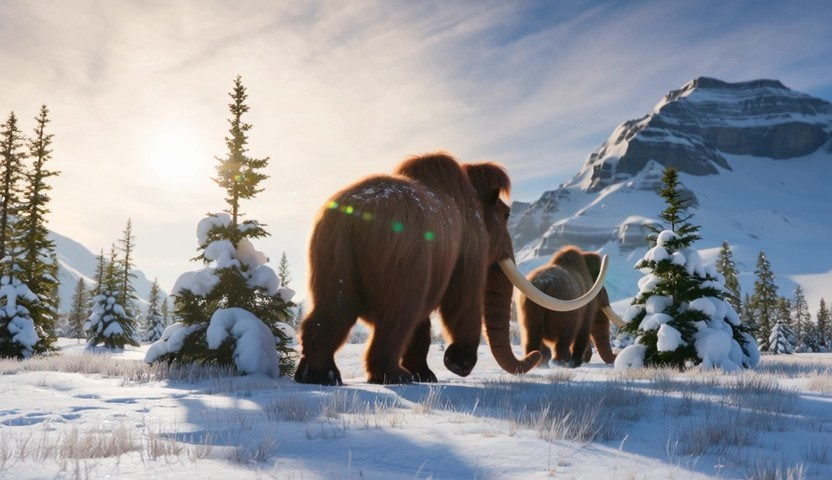
\includegraphics[width=\myimgwidth]{eccv2026/video/t2v/animal/full.jpg} &
    
\includegraphics[width=\myimgwidth]{eccv2026/video/t2v/animal/half.jpg} &
    
\includegraphics[width=\myimgwidth]{eccv2026/video/t2v/animal/inter.jpg} &
    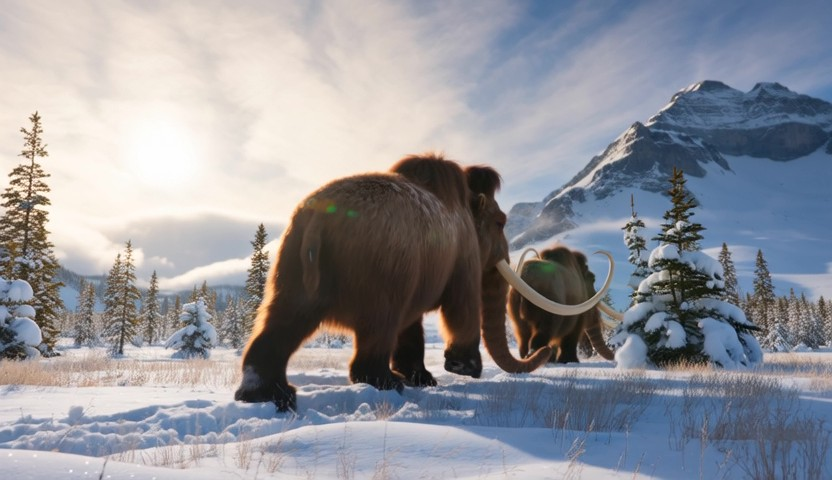
\includegraphics[width=\myimgwidth]{eccv2026/video/t2v/animal/wo_h.jpg} &
    
\includegraphics[width=\myimgwidth]{eccv2026/video/t2v/animal/wo_h_p.jpg} \\

    
\includegraphics[width=\myimgwidth]{eccv2026/video/t2v/bottle/fp16.jpg} &
    
\includegraphics[width=\myimgwidth]{eccv2026/video/t2v/bottle/full.jpg} &
    
\includegraphics[width=\myimgwidth]{eccv2026/video/t2v/bottle/half.jpg} &
    
\includegraphics[width=\myimgwidth]{eccv2026/video/t2v/bottle/inter.jpg} &
    
\includegraphics[width=\myimgwidth]{eccv2026/video/t2v/bottle/wo_h.jpg} &
    
\includegraphics[width=\myimgwidth]{eccv2026/video/t2v/bottle/wo_h_p.jpg} \\

    
\includegraphics[width=\myimgwidth]{eccv2026/video/t2v/fire/fp16.jpg} &
    
\includegraphics[width=\myimgwidth]{eccv2026/video/t2v/fire/full.jpg} &
    
\includegraphics[width=\myimgwidth]{eccv2026/video/t2v/fire/half.jpg} &
    
\includegraphics[width=\myimgwidth]{eccv2026/video/t2v/fire/inter.jpg} &
    
\includegraphics[width=\myimgwidth]{eccv2026/video/t2v/fire/wo_h.jpg} &
    
\includegraphics[width=\myimgwidth]{eccv2026/video/t2v/fire/wo_h_p.jpg} \\
  \end{tabular}
  }
  \caption{Comparison of different rotation strategies in Wan2.2 T2V models.}
  \label{fig:wan2_2_t2v}
% \vspace{-0.6em}
\end{figure*}

\begin{figure*}[!p]
  \centering
  \captionsetup{skip=1pt}
  \newcommand{\myimgwidth}{0.27\linewidth}
  \setlength{\tabcolsep}{1pt}
  {\scriptsize
  \begin{tabular}{ccc}
    
\includegraphics[width=\myimgwidth]{eccv2026/video/i2v/couple/fp.jpg} &
    
\includegraphics[width=\myimgwidth]{eccv2026/video/i2v/couple/full_h.jpg} &
    
\includegraphics[width=\myimgwidth]{eccv2026/video/i2v/couple/half.jpg} \\[1pt]

    
\includegraphics[width=\myimgwidth]{eccv2026/video/i2v/couple/inter.jpg} &
    
\includegraphics[width=\myimgwidth]{eccv2026/video/i2v/couple/w0.jpg} &
    
\includegraphics[width=\myimgwidth]{eccv2026/video/i2v/couple/wo_h_p.jpg} \\
  \end{tabular}
  }
  \caption{Comparison of different rotation strategies in Wan2.2 I2V models (top row: FP16/Full/Half; bottom row: Interleave/W/O Rot/SageAttn).}
  \label{fig:wan2_2_i2v}
% \vspace{-1.0em}
\end{figure*}

\begin{figure*}[!t]
  \centering
  \captionsetup{skip=1pt}
  \newcommand{\myimgwidth}{0.27\linewidth}
  \setlength{\tabcolsep}{1pt}
  {\scriptsize
  \begin{tabular}{ccc}
    
\includegraphics[width=\myimgwidth]{eccv2026/video/i2v/cat/fp16.jpg} &
    
\includegraphics[width=\myimgwidth]{eccv2026/video/i2v/cat/train.jpg} &
    
\includegraphics[width=\myimgwidth]{eccv2026/video/i2v/cat/train_nozj.jpg} \\
  \end{tabular}
  }
  \caption{Comparison of effect of trained Rotation (left to right: FP16, trained with orthogonality, trained without orthogonality).}
  \label{fig:train}
% \vspace{-0.8em}
\end{figure*}

The \textbf{Interleaved Rotation} method significantly improves Cosine Similarity for Wan2.2-I2V, though gains in other metrics are marginal. However, on Wan2.2-T2V, it achieves the highest Cosine Similarity and delivers substantial improvements in MSE, SSIM, and PSNR---second only to Full Rotation. For HunyuanVideo, this method achieves the best PSNR. While its performance on Wan2.2-I2V and HunyuanVideo is comparable to SageAttention, it demonstrates clear superiority on the Wan2.2-T2V model.


\textbf{Range-Optimized $\mathbf{P}$ Quantization} yields clear improvements on Wan2.2-T2V and HunyuanVideo across all metrics, yet provides marginal gains on Wan2.2-I2V. We attribute this to the I2V model's image conditioning, which constrains the attention distribution $\mathbf{P}$ to be sharply peaked (low entropy) with values concentrated near 0 and 1. In this regime, standard symmetric quantization effectively preserves the dominant structure, while range-optimized quantization can introduce subtle precision degradation. In contrast, T2V models produce more diffuse $\mathbf{P}$ distributions that benefit substantially from the full INT4 dynamic range. These findings suggest that range-optimized quantization is most beneficial for moderate-to-high entropy attention, and may be disabled for strongly conditioned, low-entropy patterns.



\paragraph{\textbf{Analysis of Rotation Strategy Differences.}}
Performance differences match RoPE-induced outlier structure: \textbf{Half Rotation} is strongest when outliers concentrate in one half-segment (I2V and HunyuanVideo), while \textbf{Interleaved Rotation} is better when local adjacent-channel correlation dominates (T2V). \textbf{Full Rotation} can over-smooth useful local structure despite stronger global redistribution.

\textbf{Practical recommendation:} For deployment on new models, we recommend \textbf{Half Rotation} as the default strategy due to its consistent performance across all tested configurations. Interleaved Rotation offers a compelling zero-cost alternative when it can be pre-fused into RoPE weights, particularly for T2V applications.



Visual inspection in Fig.~\ref{fig:wan2_2_t2v} reveals that for T2V tasks, Interleaved and Half Rotation occasionally outperform Full Rotation in specific cases. Moreover, as shown in Figs.~\ref{fig:wan2_2_t2v} and~\ref{fig:wan2_2_i2v}, both strategies exhibit clear visual superiority over the SageAttention baseline, particularly in maintaining structural integrity and temporal consistency.
 

\paragraph{\textbf{Learnable Rotation Result.}}
Learned rotation is effective \emph{only} under strict orthogonality constraints, as shown in Fig.~\ref{fig:train}; unconstrained training degrades quality (\cref{sssec:orthogonal_property}), confirming that LLM-style unconstrained rotations~\cite{liu2025spinquant,sun2025flatquant} do not transfer directly to 3D-RoPE video DiTs. With 1--2 calibration samples, orthogonal learned rotation does not outperform fixed Half Rotation.

\paragraph{\textbf{Speed and Cost Analysis.}} Our INT4 kernel yields 2.2$\times$ speedup versus custom FP16 attention, and end-to-end speedups of 1.51$\times$ (Wan2.2-I2V), 1.68$\times$ (Wan2.2-T2V), and 1.61$\times$ (HunyuanVideo). Full rotation scales linearly with sequence length, whereas attention scales quadratically. Consequently, for sequences exceeding 30k tokens, full rotation overhead remains under 1\% of attention computation. However, when paired with sparse attention on shorter sequences ($<$10k tokens), its relative overhead increases to over 10\% of the attention computation. Notably, Half Rotation reduces this overhead to approximately 3\% of the full rotation cost.


